% !TEX root = /Users/royc/Google_Drive/Thesis/RoyC_Umass_Thesis.tex
\chapter{Simultaneous analysis of multiple site alternative splicing via RNA-templated DNA-to-DNA ligation} 
\label{SeqZipPaper} 
\lhead{Chapter 2. \emph{Multiple-site alternative splicing investigation using SeqZip}}
%----------------------------------------------------------------------------------------
\section{Introduction}
	\label{SeqZipPaper:sec:Introduction}

	In eukaryotes, genome size does not scale with complexity, in large part due to expression of alternative mRNA isoforms. High-throughput sequencing has revealed that \textasciitilde58\% of Drosophila melanogaster genes and >95\% of human genes produce multiple transcripts per gene \citep{Wang2008,Pan2008,Brown2014}, with many human genes expressing 10 or more isoforms \citep{Djebali2012}. Isoform diversity is driven by alternative promoter use (i.e., alternative first exons), alternative splicing (AS) at internal sites, and alternative polyadenylation. With regard to AS, more than a quarter of human genes contain multiple alternative splicing regions separated by stretches of constitutively-included exons \citep{Fededa2005}. The combinatorial potential of such multi-site alternative splicing exponentially increases the number of possible isoforms, with some human genes predicted to have >100 isoforms and Drosophila \dscam{}, which utilizes four regions of mutually exclusive cassette exons, predicted to have 37,224!

	Although bioinformatic analysis of high throughput sequencing data has proven incredibly powerful for identifying individual alternative splicing regions and characterizing the diversity exon utilization within them, current technology is limited to \textasciitilde 500 nt of contiguous sequence. Thus complete transcripts must be intuited by piecing together multiple short reads \citep{Boley2014,Haas2013c,Grabherr2011,Garber2011a}. As a result, connectivity information present in individual mRNA molecules is lost. With regard to distal alternative splicing regions, this limits our ability to know (1) whether all possible combinations are actually produced and (2) whether there is any long-range coordination between different alternative splicing regions.

	Linked processing events have been largely observed in reporter constructs as a dependence of downstream exon inclusion due to promoter-dependent polymerase speed \citep{Kornblihtt2013}. There are also reports of coordinated endogenous exon usage \citep{Fagnani2007}, most notably for mouse Fibronectin (\fn{}) \citep{Fededa2005}. However, for many genes, including the notorious \flies{} \dscam{}, no coordination has been observed between distinct splicing decisions \citep{Miura2013b,Sun2013}. Rigorous examination of coordinated splicing remains technically challenging.

	With an end goal of thorough analysis of linked splicing decisions, we designed a novel experimental approach, SeqZip (Figure \ref{SeqZipPaper:fig:Roy2014 F1}, with which to accurately and rapidly profile multiple, distant (>1,000 nt) sites of alternative splicing contained in the same transcript. SeqZip employs RNA-templated DNA ligation of specific DNA oligonucleotides (oligos), termed ``ligamers,'' whose targeted sequences can be separated by hundreds or thousands of nucleotides. Each \textasciitilde 40 nt ligamer spans the ends of a single alternatively spliced exon, or the beginning and end of a large block of constitutively included exons, looping out the sequence in between the ends. Unique ligamer sets hybridized to individual RNA molecules are then joined by enzymatic ligation with T4 RNA ligase 2 (Rnl2) \citep{Ho2002b}. The resultant multi-ligamer product reduces the sequence space occupied by the looped out regions of the target RNA while retaining targeted exon connectivity. This connectivity can then be assessed by either size separation or sequencing of ligation products. SeqZip can quantitatively report on RNA isoform abundance, and has a usable dynamic range spanning 6 orders magnitude. Further, SeqZip does not use reverse transcriptase (RT), so is not subject to the problems associated with RT of long RNAs.

	Here we describe development and validation of SeqZip, its initial application to investigate potential connectivity among alternatively spliced exons in mouse Fibronectin (\fn{}), and its use to characterize of the immense molecular diversity of \dscam{}. We also suggest other potential applications for SeqZip, including multi-site SNP detection, multi-site smFISH probes, and Q-PCR improvements.

	\begin{figure} % Figure 1
		\centering 
		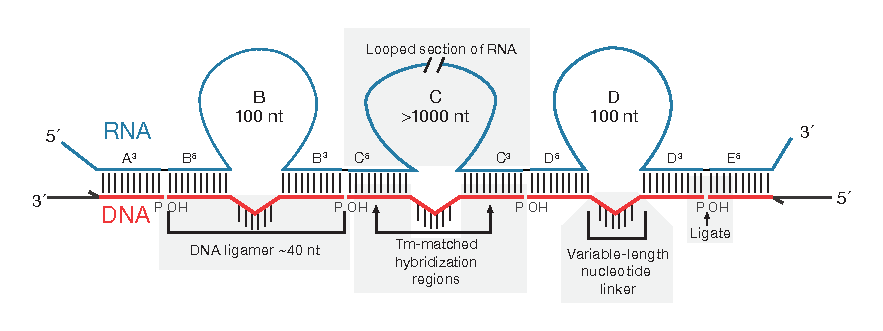
\includegraphics{Figures/SeqZipPaper/Roy2014Fig1.eps}
		\caption[Principles of the SeqZip Assay]
		{
			Principles of the SeqZip Assay\\[0.25cm]
			Using an RNA template, custom synthesized DNA oligonucleotide (``ligamers'') that have either one, or two regions of complementarity to the RNA are allowed to hybridize. Ligamers containing one region of complementarity target the terminal, flanking, constant sequences, and also contain primer sequences for subsequent amplification. Internal ligamers contain two regions of complementarity, separated by a spacer sequence. Hybridization of the internal ligamers encourages the RNA between the hybridization sites to loop out. Once all ligamers are hybridized, Rnl2 is added in excess, and the ligated DNA is amplified and analyzed.
			}
		\label{SeqZipPaper:fig:Roy2014 F1}
		\end{figure}

\section{Results}
	\label{SeqZipPaper:sec:Results}

	\subsection{Method development and validation}
		\label{SeqZipPaper:subsec: Method Development and Validation}

		The SeqZip assay requires efficient enzymatic ligation of DNA oligos hybridized to a RNA template (Figure \ref{SeqZipPaper:fig:Roy2014 F1}). Although numerous ligases can join DNA or RNA fragments hybridized a DNA template \citep{Bullard2006}, only T4 DNA ligase, and recently Chlorella virus DNA ligase, are known to previously shown to join DNA fragments hybridized to a RNA template \citep{Nilsson2001,Lohman2013c}. The commonly used T4 DNA ligase has a high proclivity for promiscuous ligation (NTL) \citep{Kuhn2005}. Therefore, we tested the ability of several other commercially available enzymes to perform ligation reactions with four or five 5\textprime~$^{32}$P-labeled 20 nt DNA oligos hybridized to adjacent positions on either a DNA or RNA template (Figure \ref{SeqZipPaper:fig:Roy2014 F2}). As expected, all DNA ligases tested [Tth DNA ligase (Thermo), Tsc DNA ligase (Prokaria), Thermostable DNA ligase (Bioline), T4 DNA ligase (NEB), and E. coli DNA ligase (NEB)] efficiently joined all four oligos hybridized to the DNA template, and Rnl2 (NEB) lacked this activity (Figure \ref{SeqZipPaper:fig:Roy2014 F2}A, left, lanes 1-6) \citep{Bullard2006}. Also as expected, T4 DNA ligase generated multiple slower migrating products, likely resulting from non-templated ligation (Figure \ref{SeqZipPaper:fig:Roy2014 F2}A, left, lane 4). When the oligos were hybridized to an RNA template, only T4 DNA ligase and Rnl2 produced ligation products (Figure \ref{SeqZipPaper:fig:Roy2014 F2}A, left, lanes 11-12). Titration of both enzymes revealed that Rnl2 had significantly higher activity on the RNA template than did T4 DNA ligase (data not shown). Further, at enzyme concentrations that yielded maximal ligation efficiencies after 8 hours, Rnl2 produced significantly less (7.5-fold) non-templated product than did T4 DNA ligase (Figure \ref{SeqZipPaper:fig:Roy2014 F2}A, right, compare lanes 9,10 and 18,19), indicating that Rnl2 has a lower propensity for promiscuous ligation. Further, the inability of Rnl2 to mediate DNA-templated DNA-DNA ligation minimizes the possibility that contaminating genomic DNA in biological samples would confound SeqZip analysis (Figure \ref{SeqZipPaper:fig:Roy2014 F2}B, left, lane 5). Therefore, we decided to move forward with Rnl2.

		\begin{figure} % Figure 2
			\centering 
			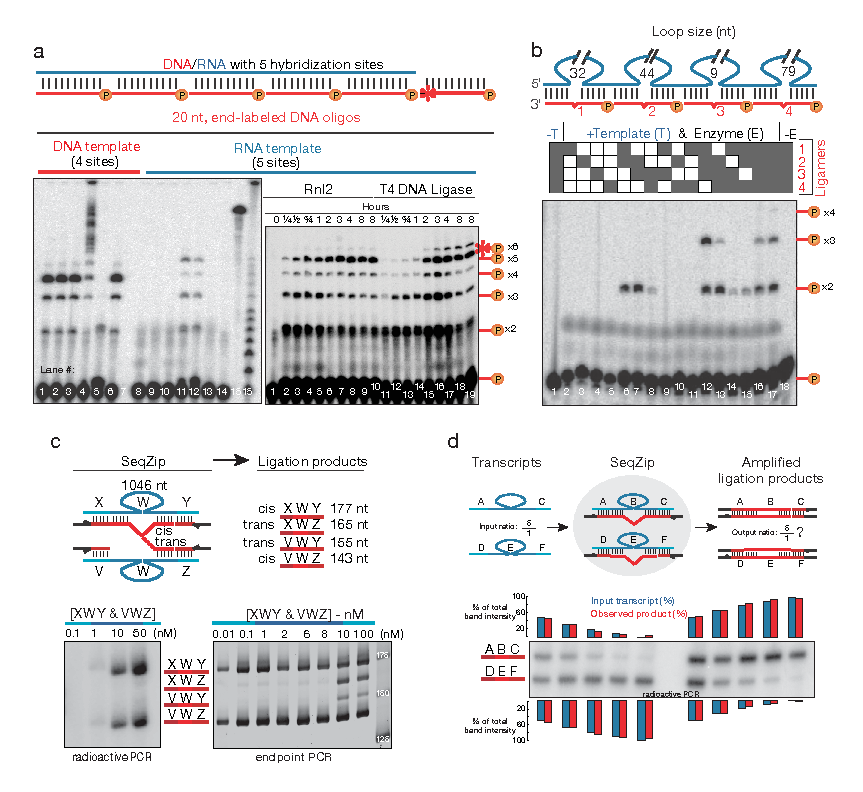
\includegraphics{Figures/SeqZipPaper/Roy2014Fig2.eps}
			\caption[T4 RNA Ligase 2 will catalyze RNA-templated DNA-to-DNA ligation]
			{
				T4 RNA Ligase 2 will catalyze RNA-templated DNA-to-DNA ligation \\[0.25cm]
				See section \ref{SeqZipPaper:figCap: Roy2014 F2} for caption
				}
			\label{SeqZipPaper:fig:Roy2014 F2}
			\end{figure}

		We next assessed the feasibility of ligating multiple DNA oligos (ligamers), each spanning a loop in an RNA template (schematized in Figure-2B). Four different ligamers were constructed to loop out various lengths of a 307 nt transcript. Each 26 nt ligamer consisted of 10 nt hybridizing to either side of the loop separated by a 6 nt spacer. Ligamers were 5\textprime~end labeled with $^{32}$P and hybridized to the template RNA individually, pairwise, in threes, or as a complete set. Ligation products were only observed when ligamers targeting adjacent RNA sequences were present in the reaction, and 4-way ligation products were obtained only when all ligamers were present. Thus DNA oligos designed to loop out various lengths of a template RNA can be used to condense the connectivity information in an RNA by more than 3 fold (i.e., a 94 nt RNA was condensed to a 26 nt DNA). In subsequent studies we were able to push this condensation ratio to >49 fold (see below).

		\subsubsection{Caption for Figure \ref{SeqZipPaper:fig:Roy2014 F2}}
			\label{SeqZipPaper:figCap: Roy2014 F2}

			T4 RNA Ligase 2 will catalyze RNA-templated DNA-to-DNA ligation

			(left) A screen of ligases was performed (see section \ref{SeqZipPaper:sec: Methods and Materials}). Ligases were incubated with an RNA or DNA template and a common pool of end-labeled DNA oligos. Importantly, the DNA template was only 80 nt long and could therefore only accommodate 4 oligos. Successful ligation is visualized as products of 40, 60, 80, or 100 nt. The doublet visible at 20 and 40 nt represents intermediate adenylated oligos. The viability of each enzyme was confirmed using the DNA template. Of note is the inability of Rnl2 to create ligation products longer than 40 nt using a DNA template. Ligases examined and venders are as follows: Lanes 1\&8) Tth DNA ligase (Thermo), 2\&9) Tsc DNA ligase (Prokaria), 3\&10) Thermostable DNA ligase (Bioline), 4\&11) T4 DNA ligase (NEB), 5\&12) T4 RNA ligase 2 (Rnl2)(NEB), 6\&13, E. Coli DNA ligase (NEB). Lanes 7\&15 were not loaded. Lane 14 contains radio-labeled oligos but no RNA template, Lane 15 contains the radiolabeled template, Lane 16 shows a 5 nt RNA ladder.
			(right) A ligation time course was performed for Rnl2 and T4 DNA ligase (section \ref{SeqZipPaper:sec: Methods and Materials}). Non-templated ligation (NTL) products are annotated as ``x-6*'' as there are only 5 hybridization sites on the RNA template.
			(b) The ability of Rnl2 to ligate adjacently hybridizing ligamers was tested by adding combinations of ligamers to individual reactions and visualizing the mobility of the ligation products on a denaturing PAGE gel. Only when adjacently hybridizing ligamers are included in a reaction are bands of the expected mobility visible. 
			(c) Four different \textit{in vitro} transcribed RNAs were created by through amplification of a plasmid with specific pairs of primers, creating a 1,163 nt RNA with unique sequences on the 5\textprime~and 3\textprime~ends. These RNAs were incubated in pairs at different concentrations, along with a pool of common ligamers hybridizing to the unique sequences and a ligamer designed to loop out the common, 1,046 nt, internal sequence. After radioactive (left) or endpoint (right), ligation products were visualized on a native PAGE gel. Trans-transcript products are not visible in radioactive PCR, are only at RNA concentrations >10 nM in the endpoint PCR analysis.
			(d) ``ABC'' and ``DBE'' RNAs were combined in different ratios (blue) in the same background of poly(A)+ RNA. Ligation product band intensity (red) was obtained by radioactive PCR.

	\subsection{Trans-transcript hybridization and ligation is minimal}
		\label{SeqZipPaper:subsec: Trans-transcript hyb and ligation}

		One concern when looping out sections of RNA is the potential for an individual ligamer to hybridize simultaneously to two different RNA molecules. This could result in the undesired formation of ligation products from intermolecular (\textit{trans}) rather than intramolecular (\textit{cis}) hybridization (Figure \ref{SeqZipPaper:fig:Roy2014 F2}C). To investigate this, we combined equimolar concentrations of two 1,127 nt RNA transcripts, each containing a common 1,106 nt internal sequence connected to unique 5\textprime~and 3\textprime~termini, with a ligamer set designed to loop out 1,046 nt of the common internal sequence (Figure \ref{SeqZipPaper:fig:Roy2014 F2}C). Following incubation with Rnl2, ligation products were PCR amplified. Ligations arising from cis-transcript hybridization result in 177 and 143 nt PCR products, whereas ligations from trans-transcript hybridization result in 165 and 155 nt PCR products. Trans hybridization efficiency should be much more sensitive to RNA concentration than cis hybridization efficiency. Consistent with this, \textit{trans} hybridization products were only abundant in endpoint PCR reactions when the two RNA targets were $\ge$10 nM, whereas \textit{cis} hybridization products were readily detectable for reactions containing as little as 0.01 nM target RNA (Figure \ref{SeqZipPaper:fig:Roy2014 F2}C, lower left). Even in samples containing 10 or 50 nM target RNA, radioactive PCR revealed that cis hybridization products predominated at low cycle numbers (Figure \ref{SeqZipPaper:fig:Roy2014 F2}C, lower left). As detailed below, both ligamer hybridization and ligation for SeqZip analysis of complex samples are carried out on magnetic beads on which poly(A) RNA derived from 5 $\mu$g of total RNA is adhered. Based on calculations of known mRNA abundances, the vast majority of cellular mRNAs are present at concentrations well below 1 nM on these beads. Thus trans hybridization is highly disfavored compared to cis hybridization under these conditions.

		To be useful for measuring the abundance of isoforms, SeqZip should faithfully recapitulate input isoform ratios. To test the ability of SeqZip to measure input isoform ratios, we combined two RNA transcripts at ratios varying from 1:1 to 1:100 (Figure \ref{SeqZipPaper:fig:Roy2014 F2}D). Output ratios determined by radioactive PCR were indistinguishable from input. With regard to dynamic range, we have obtained ligation products from as little as 903 molecules ($50 * 10^{-18}$ mole in 30 $\mu$L) of target mRNA (data not shown).

	\subsection{Reverse transcriptase-based detection versus SeqZip}
		\label{SeqZipPaper:subsec: SeqZip comparable to RT}

		As a first test of the SeqZip method for measuring relative spliced isoform abundances of an endogenous target, we chose human \cd{} (aka \textit{PTPRC}) mRNA \citep{Zikherman2008}. \cd{} is expressed in T-cells, where mRNA isoforms (R) contain various combinations of exons 4, 5, and 6 (Figure \ref{SeqZipPaper:fig:Roy2014 F3}A). Jurkat cells (resembling naïve primary T-cells) predominantly express isoforms R56, R5 and R0 (R0 denotes exclusion of all three exons) while U-937 cells (resembling activated T-cells) predominantly express R456 and R56 \citep{Yeakley2002}. These three cassette exons are adjacent to one another and together comprise only 585 nt, making this region of \cd{} mRNA amenable to analysis by both RT and SeqZip, and thus provided an excellent benchmark for comparison between methods. Whereas the RT-PCR products varied in length between 365 and 848 nt, shorter SeqZip-PCR products varied between 132 and 260 nt (Figure \ref{SeqZipPaper:fig:Roy2014 F3}B), representing a \textasciitilde 3-fold compression of the connectivity information.

		Poly(A)+-selected RNA samples from Jurkat and U-937 cells, or an equimolar combination of the two (Mix), were assessed by RT or SeqZip, both followed by radioactive PCR. Both methods reported the expected isoform profiles for every sample and relative isoform abundances reported by the two techniques were remarkably similar (Figure \ref{SeqZipPaper:fig:Roy2014 F3}C). Importantly, SeqZip did not underreport the abundance of R456 in the Mix sample (which contained all four isoforms), even though detection of R456 required three more ligation events than R0. Thus SeqZip is a robust method for detecting and quantifying spliced isoforms of endogenous transcripts. 

		\begin{figure} % Figure 3
			\centering 
			\includegraphics{Figures/SeqZipPaper/Roy2014Fig3.eps}
			\caption[SeqZip on endogenously expressed RNAs]
			{
				SeqZip on endogenously expressed RNAs\\[0.25cm]
				See subsection \ref{SeqZipPaper:figCap: Roy2014 F3} for caption.
				}
			\label{SeqZipPaper:fig:Roy2014 F3}
			\end{figure}

			\subsubsection{Figure \ref{SeqZipPaper:fig:Roy2014 F3} Caption}
				\label{SeqZipPaper:figCap: Roy2014 F3}

				SeqZip on endogenously expressed RNAs

				(a) Schematic demonstrated analysis of isoforms of the human \cd{} gene by SeqZip.
				(b) Denaturing PAGE gels showing products of RT (top) or SeqZip (bottom) \cd{} obtained from two different human T-cell lines, or a 1:1 mixture of the two.
				(c) Quantified band intensity from the gels shown in (b) (top) and a mirror image of the lane profile from the mix lanes (bottom).
				(d) When considering the cassette exons EDA (blue), and the Variable region (light blue), mouse \fn{} can produce 6 different isoforms. Isoform nomenclature used in the rest of the figure is shown next to the block schematic. Filled boxes depict exons, diagonal lines indicate isoform sequences not shown, straight lines show absence of exon in the final mRNA.
				(e) schematic showing more detail for the three regions of \fn{} AS investigated. Also shown are different ligamer pools (red). Looped regions indicated by dashed red lines, priming sequences as black arrows. 
				 (f) SeqZip was performed on poly(A)+ RNA from various \fn{} modified cell lines (see Figure \ref{SeqZipPaper:sec: Methods and Materials}). Ligation products were amplified via radioactive PCR. 
				(g) isoform band intensities are from (f) were quantified in triplicate and are plotted. Black bars indicate individual exon intensities (EDA; V-Region), or calculated expected frequencies (black bars under ``Combination pool''). Shown in light grey are observed combination isoform intensities and when available, frequencies of PacBio reads from RNA of each sample (grey). 

	\subsection{SeqZip maintains connectivity and abundance between many sites of AS}
		\label{SeqZipPaper:subsec: SeqZip Maintains Connectivity}

		Mouse Fn1 contains three well-characterized sites of AS: Extra Domain B (EDB,B), which is included in embryos but excluded in almost all adult tissues except brain; Extra Domain A (EDA (A), which displays a more variable alternative splicing pattern both across developmental stages and adult tissue types; and Variable Region (V) wherein three alternative 3\textprime~splice sites lead to 120, 95, or 0 additional amino acids in FN1 (Figure \ref{SeqZipPaper:fig:Roy2014 F3}D). One study has suggested that EDA exclusion is associated with preferential use of the most promoter-proximal 3\textprime~splice site (120) in the V region \citep{Fededa2005}. However, another concluded that splicing of the EDA and V regions occurs autonomously \citep{Chauhan2004}. These contrary results are possibly explainable by differences in both mRNA source (MEFs vs. adult tissues, respectively) and quantitation methods (region-specific or exon-specific RT-PCR, respectively).

		Together, the EDA and V regions produce up to six different spliced isoforms (Figure \ref{SeqZipPaper:fig:Roy2014 F3}D). These two alternative splicing regions are separated by constitutively included exons 34-39 comprising 815 nt. Analysis of the EDA and V exons using traditional RT-PCR generates cDNAs ranging in size from 1 to 1.6 kilobases (kb). Using SeqZip, we could compress the exon connectivity information >5-fold into uniquely sized ligation products (139 to 318 nt), greatly simplifying connectivity and abundance analysis.

		To examine possible coordination between the EDA and V regions, we first made ligamer sets that reported on each region individually (individual pools A and V) and in combination (Figure \ref{SeqZipPaper:fig:Roy2014 F3}E). Using these ligamer pools, we obtained ligation products from poly(A)+ RNA of MEF cells and analyzed them using radioactive PCR (Figure \ref{SeqZipPaper:fig:Roy2014 F3}F and G). EDA and V isoform distributions were analyzed separately or in combination (Figure \ref{SeqZipPaper:fig:Roy2014 F3}F, top row, black bars). The expected isoform distributions for all EDA and V combinations, assuming the null hypothesis of no coordination, were calculated from the individual frequencies (Figure \ref{SeqZipPaper:fig:Roy2014 F3}G, light grey bars). Connected splicing decisions should appear as deviations from null-hypothesis frequencies. In no case did the SeqZip data exhibit any significant deviance from the null hypothesis expectation. Thus, at least in primary MEFs, EDA and V region alternative splicing appears to be independently regulated.

		To directly test the effects of EDA inclusion or exclusion on splicing of the V region, \citet{Chauhan2004} used homologous recombination to create mice where the intronic splicing enhancers were modified to favor either constitutive inclusion (+/+) or exclusion (-/-) of exon 33. They also analyzed the parental strain (wt) and mice heterozygous for the modified locus (+/-). We analyzed RNA obtained from immortalized MEFs of all four genotypes using SeqZip as above(Figure \ref{SeqZipPaper:fig:Roy2014 F3}G, lower 4 rows). While we did observe constitutive inclusion or exclusion of the EDA exon as expected, in none of the lines did we observe an effect of EDA inclusion or exclusion on the V-region. We further confirmed these mRNA isoform distributions by directly sequencing full-length RT-PCR products on the PacBio platform (Figure \ref{SeqZipPaper:fig:Roy2014 F3}G, grey bars). Thus, our results are consistent with the findings of \citet{Chauhan2004} that the EDA and V regions are indeed autonomous with regard to splicing.

	\subsection{\dscam{} analysis by high-throughput sequencing}
		\label{SeqZipPaper:subsec:Dscam SeqZip Controls}

		Unquestionably, the most challenging system for measuring multi-site alternative splicing exon connectivity and isoform abundance is \dscam{} (Figure \ref{SeqZipPaper:fig:Roy2014 F4}A). \dscam{} has four regions of AS (exons 4, 6, 9 and 17), all utilizing mutually exclusive cassette exons (with 12, 47, 33 and 2 variants, respectively). Thus there are 37,224 possible \dscam{} mRNA isoforms, and previous studies have suggested that all isoforms have the potential to be generated \citep{Neves2004,Zhan2004,Sun2013}. Consistent with this, a recent study examining \dscam{} expression in individual neurons showed that all exon 4 variants are used and are incorporated in a stochastic and probabilistic manner \citep{Miura2013b}. Only one study so far has attempted to assess the extent to which specific exon choices in the different cassette regions influence one another \citep{Sun2013}. That study examined connectivity between exons 4, 6 and 9 using an RT-PCR-based method dubbed ``CamSeq''.

		\begin{figure} % Figure 4
			\centering 
			\includegraphics{Figures/SeqZipPaper/Roy2014Fig4.eps}
			\caption[Analysis of \dscam{} isoforms via High-Throughput Sequencing]
			{ 
				Analysis of \dscam{} isoforms via High-Throughput Sequencing\\[0.25cm]
				A) The \dscam{} gene. B) Triple-Read library preparation schematic. C) Rank-order expression for different \textit{in vitro} \dscam{} isoforms. Blue - \textit{in vitro} products added to libraries. with isoform identities at 4.X, 6.X, and 9.X. Red - template-switched isoforms, Yellow - ligation products created via inclusion of near-cognate ligamers. Green - \textit{in vivo} isoforms measured from S2 cells. CAM-Seq data from \citep{Sun2013}. See also Figure \ref{SeqZipPaper:fig:Roy2014 S4}. D) Schematic showing how ligamers include exon-specific barcodes. E) SeqZip application to \dscam{} isoform profiling. F) Technical and biological replicates for S2 cells. and 14-16 hr embryos using SeqZip G) Number of reads and isoforms observed per sample type. Also shared isoforms between libraries. H) Rank order isoform expression by sample type.
				}
			\label{SeqZipPaper:fig:Roy2014 F4}
			\end{figure}

		\begin{figure} % Figure S1
			\centering 
			\includegraphics{Figures/SeqZipPaper/Roy2014FigS1.eps}
			\caption[HTS Analysis of \dscam{} \textit{in vitro} transcripts]
			{
				HTS Analysis of \dscam{} \textit{in vitro} transcripts\\[0.25cm]
				 A) The similarity of sequence between cDNA, circularized cDNA, and ligation products was measured \citep{Waterhouse2009,Notredame2000}. B) The rank-order in terms of expression for different \textit{in vitro} \dscam{} isoforms is plotted. Blue dots indicate true \textit{in vitro} products added to the libraries, Red dots indiciate template-switch isoforms sequenced from, but not added to, each library. Yellow dots indicate ligation products created via inclusion of near-cognate ligamers during SeqZip ligation. Green dots indicate \textit{in vivo} isoforms measured from S2 cells using SeqZip. CAM-Seq data is from \citep{Sun2013}. See also Figure \ref{SeqZipPaper:fig:Roy2014 F4}.
				}
			\label{SeqZipPaper:fig:Roy2014 S1}
			\end{figure}

		Potentially problematic for RT-PCR-based approaches are long stretches of sequence identity in the constitutive exons separating each cluster, as well as the high sequence similarity between individual exon 4, 6 and 9 variants (Figure \ref{SeqZipPaper:fig:Roy2014 S1}). Long regions of sequence homology favor template switching during both RT and PCR \citep{Houseley2010a,Judo1998}. That is, an incompletely extended DNA strand can hybridize to a different template during the RT step or any subsequent PCR cycle, leading to novel ``switched '' isoforms not present in the original biological sample.

		To test how template switching might affect \dscam{} isoform interrogation, we developed an RT-PCR-based Triple-read sequencing method for examining exon connectivity between alternative splicing regions 4, 6 and 9, similar to CamSeq (Figure \ref{SeqZipPaper:fig:Roy2014 F4}B, \& section \ref{SeqZipPaper:sec: Methods and Materials}). To specifically assess template switching, we generated four full-length cDNA clones (\dscam{}$^{1,33,9}$, \dscam{}$^{12,32,9}$, \dscam{}$^{1,24,6}$, and \dscam$^{7,9,6}$; where the superscripted numbers indicate the included 4.X, 6.Y, and 9.Z exon variants respectively). Runoff RNA transcripts were mixed together in three different ratios (1:1:1:1, 3:3:1:1, and 5:1:1:1) and the mixtures were then processed in parallel to generate deep sequencing data. Indicative of template switching, many novel transcript isoforms containing exon combinations not present in original control transcripts were observed (Figure \ref{SeqZipPaper:fig:Roy2014 F4}C). These template-switched isoforms made up 34\% to 55\% of the total isoforms detected, with many being significantly more abundant than one or more of the input isoform(s). We next analyzed similar control data from the CamSeq study \citep{Sun2013}. CamSeq proved to be much more robust than our Triple-read protocol for accurately reporting both individual exon and individual transcript isoform abundances over five orders of magnitude. Nonetheless, template-switched isoforms were present in the CamSeq data, with many switched species being more abundant than the lowest input species. Further, many additional invasive isoforms of unknown source were detected. Although the template-switched and unknown source isoforms represented just 0.6--0.94\% of total reads, they represented 99.9\% of all isoforms detected (5,378--5,906 switched and source-unknown isoforms versus 8 input isoforms) (Figure \ref{SeqZipPaper:fig:Roy2014 S1}B). Thus, extensive template in both RT-PCR-based approaches (Triple-read and CamSeq) compromised their ability to accurately identify the exact isoform set present in the original sample and faithfully report their relative input levels.

		The technical issue of template switching can be greatly minimized using SeqZip and ligamers containing an exon-specific barcode in the linker region (Figure \ref{SeqZipPaper:fig:Roy2014 F4}D). The added sequence diversity and decreased length make SeqZip ligation products, in principle, much less prone to template switching (Figure \ref{SeqZipPaper:fig:Roy2014 S1}A). Exon-specific barcodes also ensure unambiguous isoform alignment. To apply SeqZip to \dscam{}, we designed ligamers targeting each variant exon in clusters 4, 6, and 9 plus constitutive exons 3, 5, 7--8, and 10 (97 ligamers in all) (Figure \ref{SeqZipPaper:fig:Roy2014 F4}E). Whereas the exon 3--10 region ranges in size from 1,722--1,751 nt (median = 1,734 nt) in \dscam{} mRNAs, our ligamer design compresses this \textasciitilde 5-fold to a 356 nt median-length, 7 ligamer-containing (6 ligation events) products. These products could be completely sequenced in a single Illumina MiSeq paired-end 250 nt run.

		To assess (1) maintenance of input isoform ratios, (2) template switching during PCR amplification, and (3) inappropriate ligamer hybridization during the ligation reaction, we performed control experiments containing 3 different \textit{in vitro} transcribed \dscam{} isoforms mixed at a 1:10:100 ratio in a background of total RNA from mouse Hepa 1-6 cells (Figure \ref{SeqZipPaper:fig:Roy2014 S2}A, section \ref{SeqZipPaper:sec: Methods and Materials}). Separate ligation reactions each containing a 97-ligamer pool wherein two highly expressed exons within each cluster were differently coded between the pools allowed for detection of template-switched isoforms, both in our control experiments and in biological samples. Following ligation, differentially coded samples are mixed together, subjected to PCR and sequenced (Figure \ref{SeqZipPaper:fig:Roy2014 F4}C, \ref{SeqZipPaper:fig:Roy2014 S1}B \& section \ref{SeqZipPaper:sec: Methods and Materials}).  As expected, SeqZip faithfully maintained Dscam input isoform abundance in the control samples (Figure \ref{SeqZipPaper:fig:Roy2014 S1}BB). Further, we detected no template-switched isoforms (Figure \ref{SeqZipPaper:fig:Roy2014 S1}C). Thus, as expected, our ligamer design strongly disfavors template switching during PCR amplification. This also held true for a complex biological sample (poly(A)+-selected RNA from S2 cells) where the same differentially coding approach revealed just 17 of 111,242 reads (0.015\%) corresponding to switched isoforms (Figure \ref{SeqZipPaper:fig:Roy2014 S1}C).

		\begin{figure} % Figure S2
			\centering 
			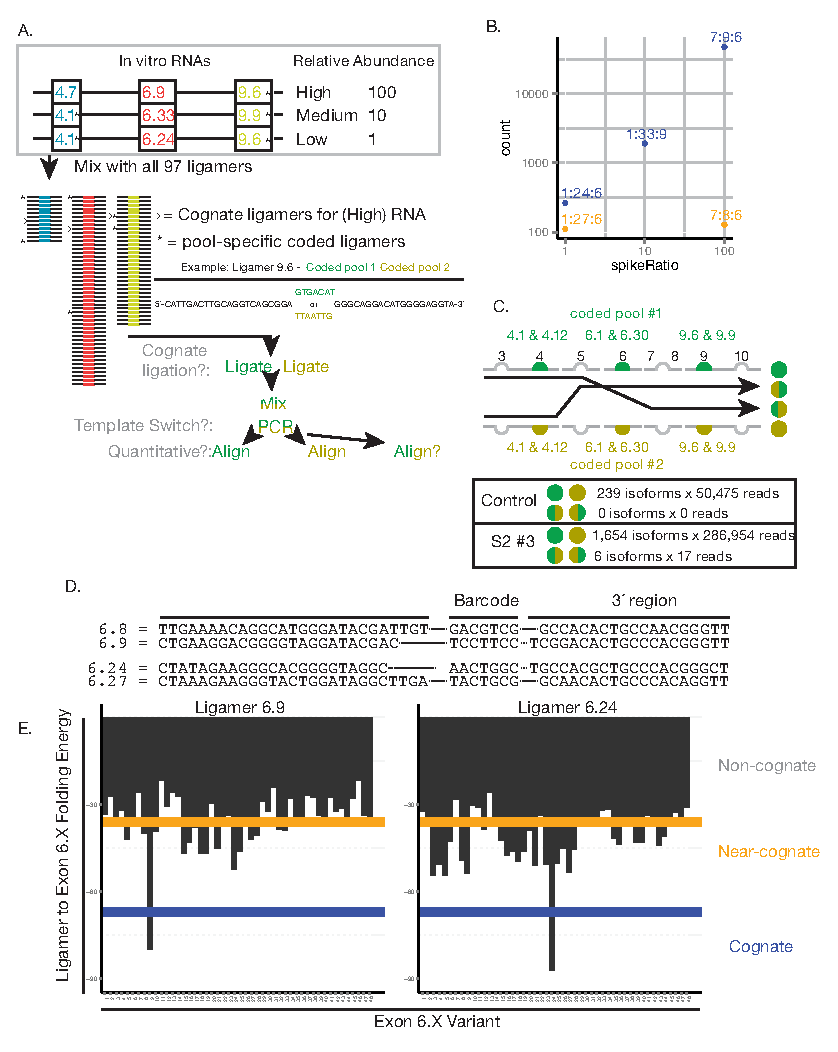
\includegraphics{Figures/SeqZipPaper/Roy2014FigS2.eps}
			\caption[SeqZip \textit{in vitro} \dscam{} controls and near-cognate ligation]
			{
				SeqZip \textit{in vitro} \dscam{} controls and near-cognate ligation\\[0.25cm]
				A) The three in vitro cDNAs used as \textit{in vitro} transcript controls. B) Expression of \textit{in vitro} controls in SeqZip analysis. Blue are true transcripts, yellow near-cognate transcripts. C) Schematic showing template-switching observation scheme. Also shown is quantified template-switched products from Control and S2 libraries. D) Comparison of E6.[8 \& 9] ligamer sequences. E) Folding energies of between ligamers 6.9 and 6.24 to all exons 6.X sequences.
				}
			\label{SeqZipPaper:fig:Roy2014 S2}
			\end{figure}

		\begin{figure} % Figure S3
			\centering 
			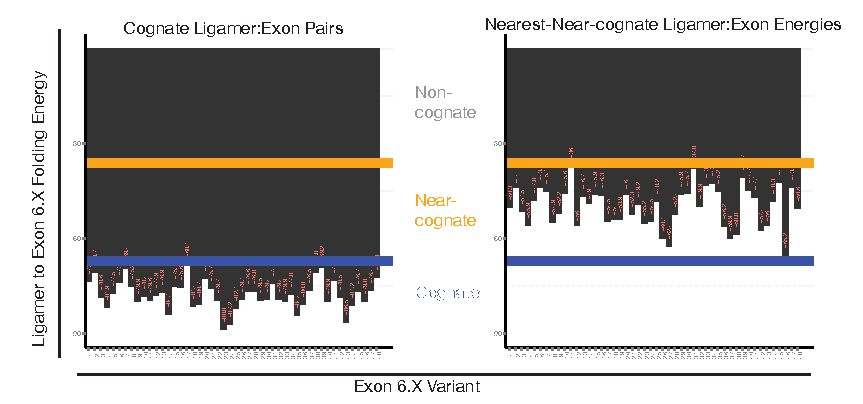
\includegraphics{Figures/SeqZipPaper/Roy2014FigS3.eps}
			\caption[Cognate and Nearest-Near cognate folding energies for \dscam{} exon 6]
			{
				Cognate and Nearest-Near cognate folding energies for \dscam{} exon 6\\[0.25cm]
				Left) Folding energies between all cognate exon:ligamer 6 pairs. Right) Nearest-NearCognate folding energies for all ligamer:exon pairs. On both Left and Right panels, Yellow line = folding energy of -36 J/mol and Blue line = -67 J/mol.
				}
			\label{SeqZipPaper:fig:Roy2014 FS3}
			\end{figure}

		Given the high sequence similarity between variant exons within each cluster, ligamer hybridization to near cognate sequences is potentially problematic. Ligamer hybridization is specified by the sequences at the ends of target exons (Figure \ref{SeqZipPaper:fig:Roy2014 F1}). To assess the potential for mis-pairing, we calculated the free energy of hybridization \citep{Reuter2010} between each ligamer and all exon variants within its target cluster. As expected, cognate ligamer-exon pairs had predicted hybridization energies lower than $\Delta G^{\circ}$ = -67 kcal/mol, with the closest near-cognate pair being at least 12 units higher (Figure \ref{SeqZipPaper:fig:Roy2014 FS3}, section \ref{SeqZipPaper:sec: Methods and Materials}). In the control samples, only 642 of 50,475 high-confidence alignments (1.3\%) contained ligamers for exons not present in any input transcript, with the vast majority of these species (221/236) being represented by 3 or fewer reads.  The two highest near-cognate hybridization products had abundances well below those of the true targets (Figure \ref{SeqZipPaper:fig:Roy2014 F4}C, \ref{SeqZipPaper:fig:Roy2014 S1}B, \ref{SeqZipPaper:fig:Roy2014 S2}D, \ref{SeqZipPaper:fig:Roy2014 S2}E), indicating that, while detectable, near-cognate hybridization is not a major problem for SeqZip.

	\subsection{Analysis of \dscam{} transcripts}
		\label{SeqZipPaper:subsec:SeqZip of endogenous Dscam}
	
		Having validated SeqZip as a reliable approach for analyzing \dscam{} isoforms, we next analyzed RNA samples from S2 cells, 4--6 and 14--16 h embryos. Between \textasciitilde 450,000--1,000,000 reads were obtained for each sample. In total, 8,397 of the possible 18,612 unique isoforms were detected (Figure \ref{SeqZipPaper:fig:Roy2014 F4}G). Individual isoform abundances were highly correlated in both technical and biological replicates (Figure \ref{SeqZipPaper:fig:Roy2014 F4}F; $r$=0.95-0.8). Of the 97 possible exons represented in our ligamer set, all were detected except 6.11, for which substantial evidence indicates it to be an unused pseudo-exon \citep{Neves2004,Zhan2004,Watson2005,Sun2013}. Thus absence of exon 6.11 reads from our libraries additionally confirms the specificity of our technique. Yet another confirmation was the individual exon utilization patterns observed in S2 cells, the only sample directly comparable between the SeqZip and CAM-Seq datasets (Figure \ref{SeqZipPaper:fig:Roy2014 FS3}A \& B). Overall, the S2 exon utilization patterns were remarkably similar between the two analyses. The exception was exon 6.47, which was well represented in the CAM-Seq data, but undetectable in the SeqZip data. We currently do not understand this failure of ligamer 6.47 to capture exon 6.47 containing transcripts. Nonetheless, the similarity between the SeqZip and Cam-Seq data with regard to all other exon abundances demonstrates the general robustness of SeqZip for accurately reporting exon abundances in highly complex samples.

		\begin{figure} % FIGURE S4
		  \centering 
		  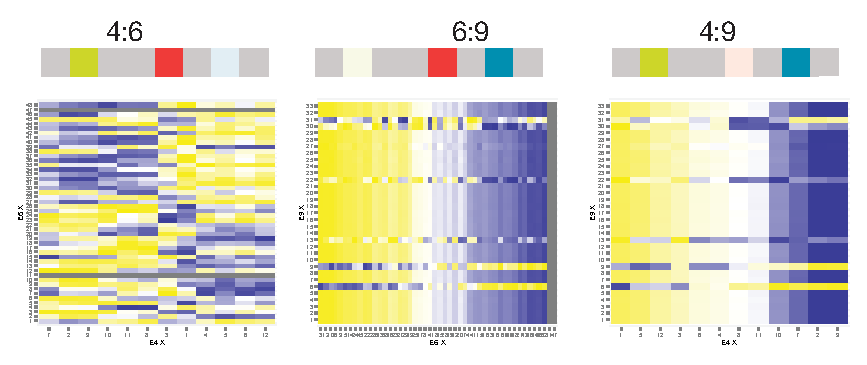
\includegraphics{Figures/SeqZipPaper/Roy2014FigS4.eps}
		  \caption[Roy et al 2014 Figure S4]
		  {Correlograms of expression for all exon pairs in \dscam{} as measured by SeqZip\\[0.25cm]
		    Pearson correlations of expression for each exon from all libraries were calculated and are plotted as shaded boxes with Yellow = $r$ of 1 and Blue = $r$ of -1.
		    }
		  \label{SeqZipPaper:fig:Roy2014 S4}
		  \end{figure}

		Comparison of exon utilization patterns across biological samples in our SeqZip data revealed a substantial increase in diversity going from S2 cells (least diversity) to 4-6 hour embryos (intermediate) to 14-16 hour embryos (highest) (Figure \ref{SeqZipPaper:fig:Roy2014 F5}A). As previously reported, the utilization patterns across clusters 4 and 9 exhibit dramatically change during development, whereas the utilization pattern across cluster 6 remains relatively static \citep{Celotto2001,Neves2004,Zhan2004,Sun2013,Miura2013b}. S2 cells are characterized by poor utilization of exons 4.[2,9], and almost exclusive utilization of exons 9.[6,9,13,30,31]. This pattern is characteristic of hemocytes \citep{Watson2005}, consistent with the macrophage-like nature of S2 cells \citep{Schneider1972}. Whereas 4-6 hour embryos are very similar to S2 cells in their cluster 4 and 9 exon utilization patterns, 14-16 hour embryos show a significant increase in exon diversity, especially in cluster 9. New isoforms are likely neuronal in origin. To compare the expression levels of hemocyte- and non-hemocytes indicative isoforms within each sample, we color coded them in the scatter plots in Figure \ref{SeqZipPaper:fig:Roy2014 F5}B. This makes it easy to see that as a class, the ``hemocyte-indicative'' isoforms (i.e., those lacking exon 4.[2,9] or containing exon 9.[6,9,13,30,31]) dominate all samples in terms of abundance. As development proceeds, however, ``non-hemocyte indicative'' isoforms increase in both number and abundance.

		For all three samples (S2 cells, 4-6 h and 14-16 h embryos), we calculated expected pairwise and triple combination frequencies in individual transcript isoforms by simple multiplication of individual variant exon frequencies in each cluster. Plotting these expected frequencies against observed frequencies (Figure \ref{SeqZipPaper:fig:Roy2014 F5}B) revealed no obvious outliers. Therefore, consistent with previous analyses \citep{Neves2004,Sun2013}, we conclude that there is no coordination between \dscam{} clusters 4, 6 and 9 with regard to alternative exon choice.
			
		\begin{figure} % FIGURE F5
		  \centering 
		  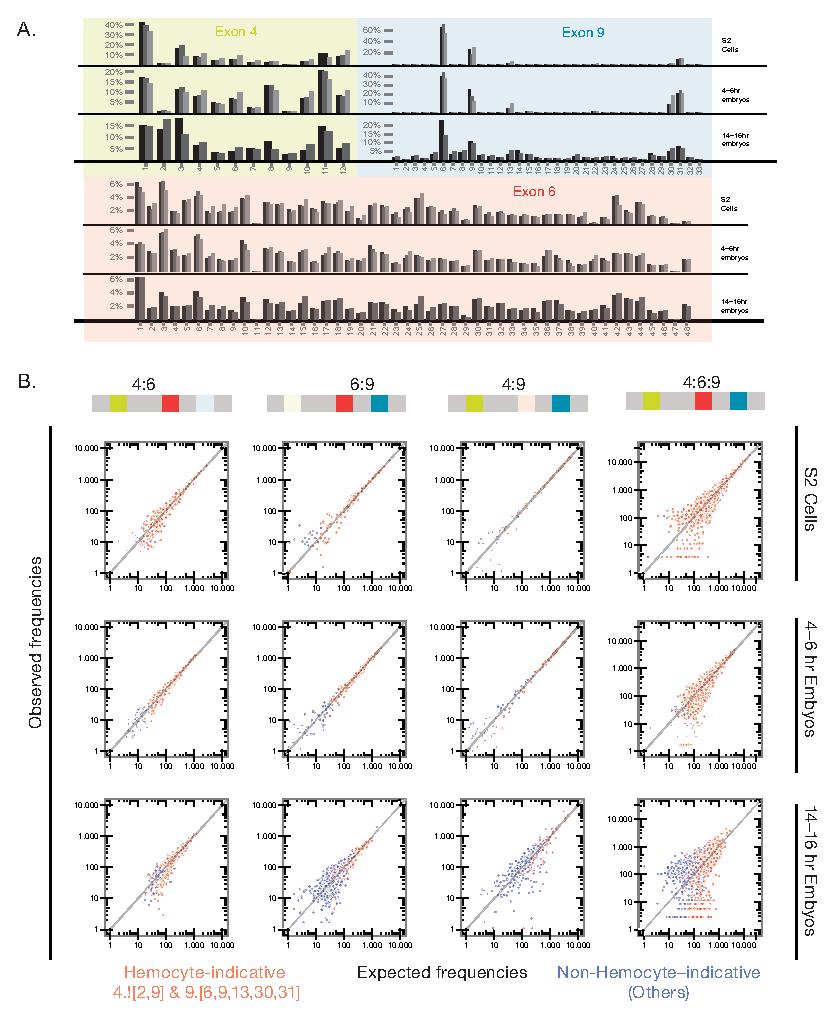
\includegraphics{Figures/SeqZipPaper/Roy2014Fig5.eps}
		  \caption[\dscam{} individual exon usage measured by SeqZip]
		  {\dscam{} individual exon usage measured by SeqZip\\[0.25cm]
		    A) Expression of each variant exon, for each library. Indivdual libraries are plotted as gray-shaded bars. B) Scatterplots showing mean Observed versus Expected individual exon abundances for the pairs, or all exon clusters (4, 6, and 9). Isoforms are colored red when hemocyte indicative or blue when not.
		    }
		  \label{SeqZipPaper:fig:Roy2014 F5}
		  \end{figure}

		\begin{figure} % FIGURE S5
			  \centering 
			  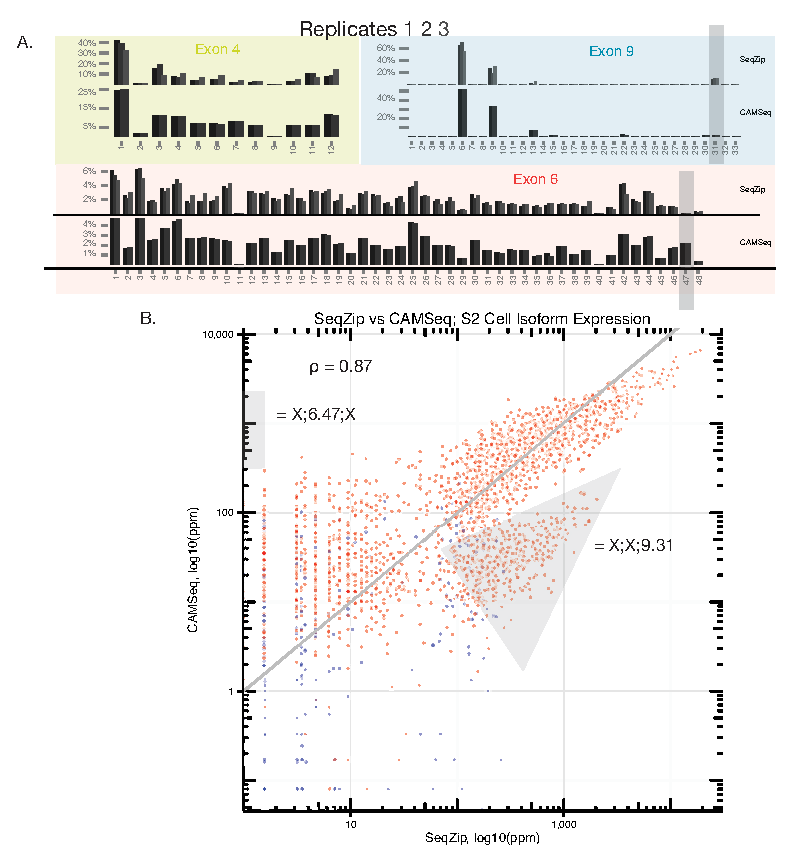
\includegraphics{Figures/SeqZipPaper/Roy2014FigS5.eps}
			  \caption[Comparison between SeqZip and CAMSeq analysis of \dscam{} isoforms in S2 cells]
			  {Comparison between SeqZip and CAMSeq analysis of \dscam{} isoforms in S2 cells \\[0.25cm]
			    A) Individual exon usages observed for S2 cells observed using either SeqZip (Top) or CAMSeq (Bottom). 
			    }
			  \label{SeqZipPaper:fig:Roy2014 FS5}
			  \end{figure}

\section{Discussion}
	\label{SeqZipPaper:sec:Discussion}

	Here we describe development and implementation of a new method, SeqZip, for compressing sequence information of long RNAs while maintaining connectivity between distant regions of individual molecules. Completely orthogonal to traditional methods of RNA sequence investigation such as RT-PCR, SeqZip can be used to quickly and efficiently examine complex alternative splicing events, and is particularly useful for investigating genes harboring multiple distal sites of AS. Using SeqZip to investigate the splicing coordination in mouse \fn{} transcripts and in \flies{} \dscam{} we found no evidence of splicing coordination in either gene. 

	\subsection{Deconvoluting \dscam{}}

		Many of the \dscam{} variant exons arose from exon-duplication and, therefore, have very high sequence similarity \citep{Lee2010b}. The extreme diversity of \dscam{} has been implicated in important biological functions, including neuronal self recognition and immune function \citep{Wojtowicz2004,LawrenceZipursky2013,Watson2005}. While flies coding for 4,752 unique isoforms have been shown to display equivalent neurite formation as wild-type controls, animals expressing 1,152 isoforms display neuronal branding defects, supporting the view that diversity of molecules, and not sequence, is essential for biological function \citep{Hattori2009}.

		Multiple technical hurdles currently hamper characterization of \dscam{} isoforms: (1) determining the relative utilization of individual exons within each cassette region, while maintaining connectivity information between cassettes using current Illumina-platform RNA-Seq read lengths is currently not possible \citep{Neves2004,LawrenceZipursky2013,LeGault2013}; (2) sequencing full-length mRNAs expressed across 5 orders of magnitude is technically challenging and costly \citep{Hattori2008,Sharon2013}; and (3) due to sequence similarity between \dscam{} isoforms, template switching artifacts complicate high-throughput sequencing library preparation.

		Recently, two studies have lent additional support to a longstanding hypothesis that \dscam{} isoforms are produced via stochastic processing. The first is an elegant genetic investigation into exon 4 variants, demonstrating that changes in variant expression are not due to any requirement at a specific time, cell, or tissue, and instead is determined by modulating the probability of choosing certain variants \citep{Miura2013b}. In the second study, \citet{Sun2013} employed a novel high throughput sequencing approach (CAMSeq). CAMSeq begins by amplifying barcoded 2 kb \dscam{} RT products circularized into \textasciitilde 1 kb inserts containing exon clusters 4, 6 and 9. Circularized products are amplified again, and deep sequenced via sequential hybridization of three constitutive exon-specific primers, sequencing exons 4, 6, and 9. CAMSeq is extremely similar to the Triple-read approach described above. CAMSeq analysis of \dscam{} diversity in multiple \flies{} (S2 cells, embryos, larva, pupae, and adult brains) led the authors to conclude that all possible isoforms are expressed at all developmental stages, again in a stochastic fashion.

		Two potential complications of the CAMSeq approach are: (1) chimera formation via intermolecular ligation during the circularization step, and (2) template switching during the RT step or either round of PCR. Using a clever barcoding scheme, the authors were able to determine that chimeras represented \textasciitilde1\% of their CAMSeq libraries, indicating that this is a non-trivial problem. Indeed, in control libraries made from a mixture of 8 \textit{in vitro} transcribed \dscam{} isoforms, chimera formation resulted in detection of >5,000 other isoforms not present in the original mix, with \textasciitilde 500 being represented by $\ge$ 10 reads (Figure \ref{SeqZipPaper:fig:Roy2014 S1}B).

		Whereas barcoding can distinguish bona fide isoforms from chimeras, there is no way to distinguish isoforms present in the original RNA sample from artificial combinations created by template switching. Template switching can occur during the initial RT step \citep{Houseley2010a}, or during either PCR amplification step \citep{Meyerhans1990a,Judo1998}. With these potential experimental complications in mind, we decided to investigate and characterize isoforms of \dscam{} using the SeqZip method.

		Our analysis of \dscam{} yielded a very similar exon usage frequency to that of CAMSeq at each stage examined (Figure \ref{SeqZipPaper:fig:Roy2014 FS5}). Additionally, we also observed no connectivity between exon choices from any of the three clusters (Figure \ref{SeqZipPaper:fig:Roy2014 F5}B). We do observe increased exon 9 diversity in 14-16 h embryos. Taken together, our data also support the view that flies use a complex mixture of \dscam{} isoforms, produced via stochastic and probabilistic splicing, in order to discriminate self from non-self neuronal processes \citep{LawrenceZipursky2013}.

		Even a relatively shallow analysis of the human transcriptome using single-molecule sequencing on the PacBio platform has revealed a rich population of previously unreported isoforms, and thorough analysis of complex spliced genes is becoming a reality \citep{Sharon2013}. However, the most interesting spliced genes often produce long ($>$1,500 nt) transcripts that are often expressed in the central nervous system \citep{Park2007}. While human \textit{Dscam} does play a role in the neurologically disorder down syndrome, it does not undergo extensive splicing \citep{Yamakawa1998a}. Unlike \textit{Dscam}, human \textit{protocadherin} and \textit{neurexins} are heavily processed and, similar to \dscam{}, are involved in neuronal wiring \citep{Ushkaryov1992,Wu1999}. Recently, PacBio was used to rigorously determine neurexin gene isoforms, and found that these genes do produce many different isoforms, but lack any coordination in their alternative processing events \citep{Treutlein2014}. Perhaps efficient cell-cell recognition is accomplished not by an ordained and complicated system, but by random and frequent shuffling of exons.

	\subsection{Other applications of SeqZip}

		A potentially more routine use of the SeqZip methodology is highlighted by our analysis of mouse \fn{}, where we simultaneously measured 12 different alternative splicing isoforms and determined their relative expression using traditional PAGE. While it is intriguing to think that inclusion of the EDA exon in this gene influences alternative splicing decisions over a kilobase and multiple exons away, we saw no evidence for this type of regulation in any of the cell lines investigated.

		SeqZip could also be used to assess the integrity of long RNAs, extended 3\textprime~UTRs \citep{Wang2013b}, or piRNA-precursor transcripts \citep{Li2013h}. A more routine laboratory task where SeqZip could prove useful is Q-PCR. SeqZip does not include an RT step, providing an orthogonal means of measuring RNA abundance. Also, any sequence can be placed between each ligamers two regions of complementarity. Therefore sequences for custom priming, restriction digestion, recombination, etc., can be introduced allowing for quantification or manipulation of ligation products. Analysis of ligation products can even be multiplexed, allowing for simultaneous generation and analysis of internal controls and primer sets. As demonstrated by our \dscam{} study, SeqZip ligation products can be analyzed with high-throughput sequencing via incorporation of platform-appropriate priming sequences either in the terminal PCR primers, or in the spacer sequences of the internal ligamers. Therefore, this robust methodology, which only takes 1.5 days to complete, complements more traditional analysis via RT-PCR. 

\section{Materials and Methods}
	\label{SeqZipPaper:sec: Methods and Materials}

  \begin{description}
  	\item[Cell lines and Drosophila melanogaster stocks] \hfill 
		
		U-937 (CRL-1593.2), Jurkat (TIB-152), and S2 (CRL-1963) cell lines were obtained from ATCC. Primary MEF cells were from C57BL/6J strain background and were obtained from The Jackson Labs. MEF lines were immortalized using SV40 retroviral infection. Mixed Drosophila melanogaster Oregon-R males and females were maintained at 25$\,^{\circ}\mathrm{C}$. Embryos 4-6 hour, and 14-16 were collected. 

		\item[Ligamer design] 
		The 5\textprime~and 3\textprime~most sequences of a target sequence (ex. exon or multiple exons) were obtained from online databases (Ensembl, UCSC, etc.). The \textit{T}$_{m}$ of these sequences was normalized to 60$\,^{\circ}\mathrm{C}$ $\pm$ 5$\,^{\circ}\mathrm{C}$ according to nearest-neighbor rules \citep{Xia1998} by adding or removing flanking nucleotides. Most regions of complementarity fell 12--25 nt in length. After assembling complementary region sequences, matching sequences (i.e. the 5\textprime~and 3\textprime~edge sequences of a specific exon) were combined with a short spacer sequences included between them. For this study the spacer was restricted to (TGA)*N, where N was typically 2. With the full sequence now assembled, the reverse complement was taken, ligamers requiring 5\textprime~phosphorylation for subsequent ligation were marked, and ligamers were ordered in 96 well format from Integrated DNA Technologies (IDT). Ligamers were reconstituted to 1 $\mu$M in sets targeting specific regions on a specific gene and subsequently diluted further for use in the SeqZip protocol.

		\item[SeqZip] 
		Total RNA was isolated from a cell line or tissue type using Tri Reagent (MRC) according to the manufacturer's instructions. Poly(A)+ RNA was isolated using the Poly(A)Purist MAG kit from Ambion (AM1922). Poly(A)+ RNA was not eluted from magnetic beads, and after the last wash step, beads were aliquoted into appropriate amounts and reconstituted in hybridization buffer (60 mM Tris-HCl pH 7.5 @ 25$\,^{\circ}\mathrm{C}$, 1.2 mM DTT 2.4 mM MgCl$_{2}$, 480 $\mu$M ATP) including 10 nM appropriate ligamers. Hybridization was performed in a thermocycler by heating samples to 62$\,^{\circ}\mathrm{C}$ for 5 minutes and cooling to 45$\,^{\circ}\mathrm{C}$ in 3$\,^{\circ}\mathrm{C}$ by 10 minute increments. Samples were left at 45$\,^{\circ}\mathrm{C}$ for 1 hour, then cooled again in 3$\,^{\circ}\mathrm{C}$ by 10 minute increments until 37$\,^{\circ}\mathrm{C}$ was reached, followed by enzyme addition. T4 RNA ligase 2 (NEB, M0239) was added to compose 10\% of final volume (ex. 2.5 $\mu$l in 22.5 $\mu$L previous samples). At this point the samples were in 1X ligation buffer (51 mM Tris-HCl pH 7.5 @ 25$\,^{\circ}\mathrm{C}$, 2.01 mM DTT, 5 mM KCl, 2 mM MgCl$_{2}$, 400 $\mu$M ATP, 3.5 mM (NH$_{4}$)$_{2}$SO$_{4}$, 5\% glycerol). Samples were incubated at 37$\,^{\circ}\mathrm{C}$ for 8--16 hours. Ligation products were amplified by PCR and analyzed by either native PAGE or sequencing.

		\item[PacBio FN1 Analysis] 
		cDNA prepared using primers designed to amplify EDB->IIICS region was submitted for library construction using ``The DNA Template Prep Kit 2.0 ''and sequenced on a PacBio RS II. Circular Consensus reads were aligned to an index of FN1 isoforms using BLAT. 

		\item[MiSeq Library Preparation] 
		Individual SeqZip ligation reactions were amplified for 12 cycles using common primers, in individual PCR reactions. After amplification, PCR reactions were run on a 5\% acrylamide gel, and DNA in the appropriate size range of full-length ligation products was cut from the gel, and eluted. Eluted DNA was precipitated, and amplified for another 22 cycles using primers containing Illumina priming sequences with integrated barcodes. These PCR reactions were cleaned using a PCR clean up kit (Qiagen) and quantified. Samples were mixed and submitted for sequencing on the MiSeq instrument, paired-end 250 nt read option.

		\item[MiSeq Library Analysis] 
		Paired reads were split according to the index read. Libraries were aligned against an index of all possible \dscam{} ligamer arrangements using bowtie2 \citep{Langmead2012} in the ``-very-sensitive-local'' mode and constrained using ``-no-discordant'' to only look for reads where both pairs aligned to the same isoform. Read counts per isoform were extracted using the SAMtools software package \citep{Li2009d}. Analysis of count values and graph generation was performed using R \citep{RDevelopmentCoreTeam2011}.
		
		\item[Triple Read Sequencing] 
		To interrogate, RNA samples, reverse transcription was performed using 5 $\mu$g total RNA, Superscript II (Invitrogen) and random hexamer at 42o C for one hour. Three strand-switching control experiments were performed by mixing plasmids encoding isoforms \dscam{}$^{1.33.9}$, \dscam{}$^{12.32.9}$, \dscam{}$^{1.24.6}$, and \dscam{}$^{7.9.6}$ in the ratios of 3:3:1:1, 1:1:1:5, and 1:1:1:1. PCR primers specific to exon 3 (Not1Ex3For: TAT CGG CGG CCG CGG ACG TCC ATG TGC GAG CCG) and exon 10 (Ex10RevNot1: ATA TCG CGG CCG CGA GGA TCC ATC TGG GAG GTA) with a Not I restriction enzyme site on the 5\textprime~ends were used to amplify the cDNA or plasmids containing the region encompassing exons 4, 6, and 9 using Phusion polymerase (NEB) with an annealing temperature of 55$\,^{\circ}\mathrm{C}$ and 1 minute extension. PCR products were gel purified and digested with Not1 for 2 hours at 37$\,^{\circ}\mathrm{C}$, followed by a heat inactivation at 65$\,^{\circ}\mathrm{C}$ for 20 minutes. 0.5 $\mu$g of the digested PCR products were circularized in 500 $\mu$L 1X T4 ligase buffer (NEB) with 1 $\mu$l T4 ligase at 18$\,^{\circ}\mathrm{C}$ overnight. Inverse PCR was then performed with primers specific to exons 7 (PEex7Rev:CAA GCA GAA GAC GGC ATA CGA GAT CGG TCT CGG CAT TCC TGC TGA ACC GCT CTT CCG ATC TAT GAA CTT GTA CCA T) and 8 (PEex8For: AAT GAT ACG GCG ACC ACC GAG ATC TAC ACT GTT TCC CTA CAC GAC GCT CTT CCG ATC TAA GTG CAA GTC ATG G) that containing Illumina paired-end clustering sequences using Phusion polymerase (NEB) with a 55$\,^{\circ}\mathrm{C}$ annealing temperature and 30 second extension. Libraries were gel purified, quantified and clustered on a Genome Analyzer IIx paired-end flow cell on an Illumina cluster station using the standard clustering protocol.

		Sequencing was performed on an Illumina GAIIx by modifying the protocol for paired-end sequencing with an index read. Briefly, read 1 was performed for 24 cycles with a primer complementary to the 5\textprime~end of exon 8 (Ex8For:ACG ACG CTC TTC CGA TCT AAG TGC AAG TCA TGG). The flow cell was denatured to remove the exon 9 sequencing products, a primer complementary to exon 3 (Ex3For:CCC GGG ACG TCC ATG TGC GAG CCG) was annealed, and read 2 sequenced for 12 cycles. Next, the flow cell was re-clustered using the paired-end protocol and read 3 performed for 20 cycles using a primer complementary to exon 7 (Ex7Rev:GAA CCG CTC TTC CGA TCT ATG AAC TTG TAC CAT).

		Base calling was performed from the raw images using the Firecrest, Bustard, and Gerald software modules of GAPipeline-1.4.0 and a matrix.txt file for a PhiX lane from a previous flow cell for calibration. This generated a single FastQ file per lane containing the three reads from each cluster concatenated together. The reads within the FastQ files were parsed to separate the three reads and the identity of each exon within each cluster, and thus the full isoform, determined by matching to a database of known exon sequences using Perl scripts.
		
		\item[Determining Sequencing Similarity of \dscam{} Sequences] 
		Endogenous \dscam{} sequences were obtained from genomic build DM3 using BEDTools \citep{Quinlan2010}. All possible \dscam{} were assembled using a PERL script. Five hundred random isoforms were obtained, and aligned using TCOFFEE \citep{Notredame2000} in the Jalview package \citep{Waterhouse2009}. Consensus scores of alignments were exported and graphed in R. The same analysis was performed on \dscam{} ligation products, except ligamer sequences were used in place of endogenous exonic sequences.
		
		\item[Trans-transcript RNA design] 
		PCR was performed using oligos specified in Table S2 in desired combinations. These oligos have partial complementarity to the open reading frame (ORF) of human eiF4A3. A plasmid containing this ORF was used (RefSeq: NM_014740 ) as a template for PCR. The sequences of the individual RNAs were confirmed by sequencing. 

		\item[Reverse Transcription] 
		Reverse transcription was performed using SuperScript III (Invitrogen), 200 ng poly(A) selected RNA, and either a gene-specific antisense primer or anchored oligo(dT).

		\item[Radioactive PCR] 
		A 5\textprime~$^{32}$P-radiolabeled antisense primer was used in PCR reactions run for a limiting number of PCR cycles. Multiple cycle numbers were performed to test for expected increases in signal (typically 15,18, and 21 cycles). Reactions analyzed on denaturing acrylamide gels to size resolve ligation products. Bands were quantified using a Typhoon imager (GE Healthcare) and the ImageQuant software package (GE Healthcare).

		\item[Endpoint PCR] 
		Using a 25 $\mu$l reaction volume, after 8 hours of ligation, 2 $\mu$l reaction volume was added into a 20 $\mu$l PCR reaction with 500 nM primers and 50\% Green master mix from Promega. Samples were amplified for 35 cycles using a hybridization temperature 5$\,^{\circ}\mathrm{C}$ below the \textit{T}$_{m}$ of the primers. 10 $\mu$l of each PCR reaction was run out on an appropriate percentage native 29:1 (acrylamide: bis-acrylamide) native acrylamide gel.

		\item[Statistical Analysis] 
		Error bars represent the standard error of the mean of the experimental replicates. Errors were propagated from individual standard deviations according to the formula $\Delta$Z = Z(SQRT((($\Delta$A/A)^2)+(($\Delta$B/B)^2))) where Z = A/B.

		\end{description}

\section{End Matter}
	\label{SeqZipPaper:sec:End Matter}

	\begin{description}

		\item[ACKNOWLEDGEMENTS] 
		Alper Kucukural for bioinformatics support. Kristen Lynch and Eric Shuman for plasmids. Andrés Muro for Fn1 cell lines. 

		\item[AUTHOR CONTRIBUTIONS] 
		CKR, BRG, PDZ, and MJM conceived the experiments. CKR and SO performed the experiments and conducted the analysis. CKR, PDZ, and MJM wrote the paper. 

		\item[COMPETING FINANCIAL INTERESTS] 
		The authors have applied for a patent (12/906,678) concerning the SeqZip protocol. 

		\end{description}

\cleardoublepage